Plutchik proposed a psychoevolutionary classification approach for general emotional responses. He considered there to be eight primary emotions—anger, fear, sadness, disgust, surprise, anticipation, trust, and joy.
He also created a wheel of emotions to illustrate different emotions. Plutchik first proposed his cone-shaped model (3D) or the wheel model (2D) in 1980 to describe how emotions were related \cite{enwiki:1136521972}.
\begin{figure}[H]
	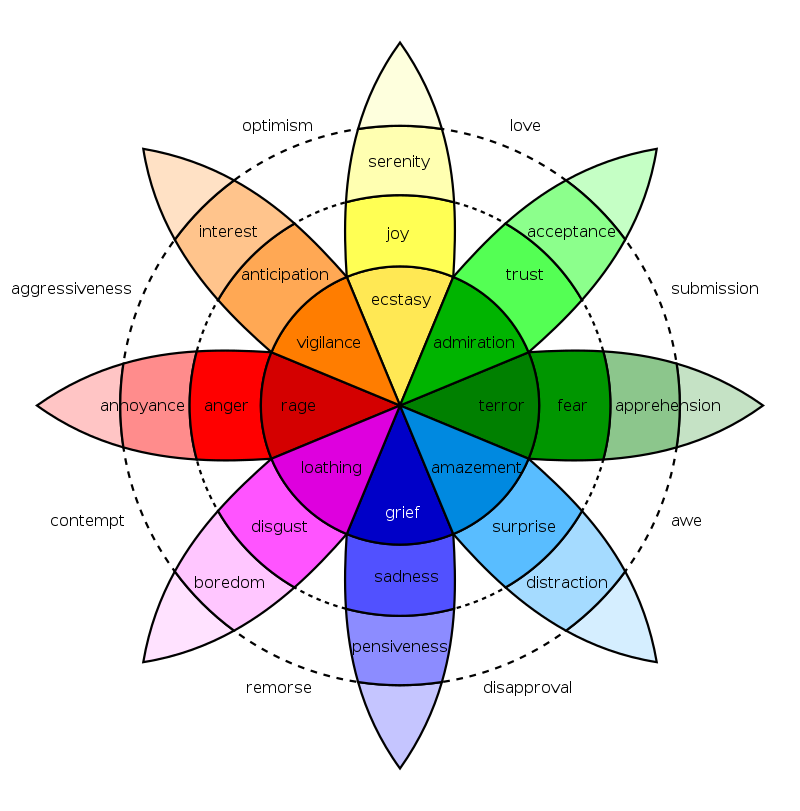
\includegraphics[width=\columnwidth, keepaspectratio]{Plutchik'sWheelofEmotions}
	\caption{Plutchik's Wheel of Emotions}
	\label{Fig:fig}
\end{figure}
Figure \ref{Fig:fig} shows PWOE.